\documentclass[pre, a4paper, aps, floatfix, superscriptaddress, onecolumn, notitlepage, longbibliography]{revtex4-1} %hyperref

\usepackage[utf8]{inputenc}
\usepackage[T1]{fontenc}

%\usepackage{float}
\usepackage{amssymb, amsmath, amsfonts}  %amssymb, amsmath, amsfonts
\usepackage{graphicx}
\usepackage{todonotes}

\usepackage[rmargin=20mm, tmargin=20mm, bmargin=20mm, lmargin=60mm]{geometry}

\frenchspacing

\newcommand{\THP}{\affiliation{Institute for Theoretical Physics, University of Cologne, 50937 K\"oln, Germany}}
\newcommand{\FZJ}{\affiliation{Forschungszentrum J\"ulich, Institute for Energy and Climate Research - Systems Analysis and Technology Evaluation (IEK-STE), 52428 J\"ulich, Germany}}


\begin{document}

\title{Multifractal Detrended Fluctuation Analysis}


\author{Leonardo Rydin Gorj\~ao}
\email{\texttt{l.rydin.gorjao@fz-juelich.de}}
\FZJ \THP

\begin{abstract}
Multifractal Detrended Fluctuation Analysis in Python
\end{abstract}

\maketitle

%%%%% Beginning of the main text %%%%%

\section*{Summary}
A common tool to unveil the nature of the fractionality of a process, natural or computer-generated, is the Detrended Fluctuation Analysis (DFA), initally developed by Peng \textit{et al} and later extended to study multifractal processes by Kandelhardt \textit{et al}, giving rise to Multifractal Detrended Fluctuation Analysis (MFDFA) \cite{Peng1994,Kantelhardt2002}.
It addresses the question of the presence of long-range correlations and can be employ to study discrete processes, as auto-regressive models, as well as time-continuous stochastic processes.
An extensive study of DFA and the interplay between trends in data and correlated noise can be found in \cite{Hu2001}.

In order to determine the self-affinity of a stochastic process, one can study the relation between the variance of the process and time.
Auto-regressive and stochastic processes diffuse with different rates, and uncovering the rates of diffusion is of importance in natural processes with power-law correlations, like temperature variability \cite{Meyer2019} earthquake frequency \cite{Shadkhoo2009}, heartbeat dynamics \cite{Ivanov1999}.
Fluctuation Analysis provides a method to uncover these correlations, but fails in the presence of trends in the data, which is, for example, particularly present in weather and climate data.
Detrending the data via polynominal fittings allows one to uncover solely the relation between the inherent fluctuations and the time scaling of a process.
Moreover, several processes might be driven by more than one time scale.
They might be of a mono- or multi-fractal nature.
By studying a continuum of power variations of the Detrended Fluctuation Analysis one extends into Multifractal Detrended Fluctuation Analysis, which permits the study of the fractality of the data by comparing power variations of Detrended Fluctuation Analysis, see below.

There are currently no flexible and available implementations of Multifractal Detrended Fluctuation Analysis in python, but there are several Matlab versions available.
There is a particularly thorought introductory guide to Multifractal Detrended Fluctuation Analysis, and subsequently a source-code by Espen Ihlen from 2012~\cite{Ihlen2012}, which is flexible but slow.
With this implementation, efficiency was sought, by making the most out of Python, reshaping the code to allow for multithreading, especially relying on \texttt{numpy}'s \texttt{polynomial}, which scales easily with modern computers having more CPU cores.

\section*{Theory}
Multifractal Detrended Fluctuation Analysis studies the fluctuation of a given process by considering increasing segments of the timeseries.
Take a timeseries $X(t)$ with $N$ elements $X_i$, $i=1,2, \dots, N$.
Obtained the ``detrended'' profile of the process by defining
\begin{equation}
  Y_i = \sum_{k=1}^i \left ( X_k - \langle X \rangle \right),~\text{for}~i=1,2, \dots, N,\nonumber
\end{equation}
i.e., the cumulative sum of $X$ subtracting the mean $\langle X \rangle$ of the data.
Section the data into smaller non-overlapping segments of length $s$, obtaining therefore $N_s = \text{int}(N/s)$ segments.
Given the total length of the data isn't always a multiple of the segment's length $s$, discard the last points of the data.
Consider the same data, apply the same procedure, but discard now instead the first points of the data.
One has now $2N_s$ segments.

To each of this segments fit a polynomial $y_v$ of order $m$ and calculate the variance of the difference of the data to the polynomial fit
\begin{equation}
  F^2(v,s) = \frac{1}{s} \sum_{i=1}^s [Y_{(v-1)s + i} - y_{v,i}]^2, ~\text{for}~v=1,2, \dots, N_s,\nonumber
\end{equation}
where $y_{v,i}$ is the polynomial fitting for the segment $i$ of length $v$.
One also has the freedom to choose the order of the polynomial fitting.
This gives rise to the denotes \texttt{DFA1}, \texttt{DFA2}, \dots, for the orders chosen.

Notice now $F^2(v,s)$ is a function of each variance of each $v$-segment of data and of the different $s$-lenght segments chosen.
On can now define, will all due generally, the $q$-th order fluctuation function by averaging each row of segments of size $s$
\begin{equation}
  F_q^2(s) = \left\{\frac{1}{N_s} \sum_{v=1}^{N_s} [F^2(v,s)]^{q/2}\right\}^{1/q}\nonumber
\end{equation}
where Detrended Fluctuation Analysis with $q=2$ is a subset of Multifractal Detrended Fluctuation Analysis (where $q\in \mathbb{R}$).
The $q$-th order fluctuation function $F_q^2(s)$ is our object of interest.

The inherent scaling properties of the data, is the data displays power-law correlations, can now be studying in a log-log plot of $F_q^2(s)$ versus $s$, where the scaling of the data obeys a power-law with exponent $h(q)$ as
\begin{equation}
  F^2(s) \sim s^{h(q)},\nonumber
\end{equation}
where $h(q)$ is the \textit{self-affinity} exponent, which may dependent on $q$, and relates to the previously introduced Hurst exponent.
The self-affinity exponent $h(q)$ is calculated by finding the slope of this curve in the log-log plots, as seen henceforth in the figures.

If the data is monofractal, the \textit{self-affinity} exponent $h(q)=h$ is independent of $q$.
On the other hand, if the data is multifractal, the dependence on $q$ can be understood by studying the multifractal scaling exponent $\tau(q)$ \cite{Barabasi1991}
\begin{equation}
  \tau(q) = qh(q) - 1.\nonumber
\end{equation}
For a clearer discussion of these properties, see \cite{Kantelhardt2002,Barabasi1991}.


\section{Examples}

To exemplify the usage of Multifractal Detrended Fluctuation Analysis, take two common examples of stochastic processes, a continuous-time stochastic process: fractional Ornstein--Uhlenbeck process and a discrete auto-regressive process:

For an example of multifractal behaviour in real-world data of sun spots timeseries, alongside a detailed explanation of MFDFA, or an application to European temperature variability, see respectively \cite{Movahed2006} and \cite{Meyer2019}.

To study the scaling effects in continuous stochastic processes, three exemplary fractional Ornstein--Uhlenbeck processes are taken, given by
\begin{equation}
  dX_t = - \theta X_t dt + \sigma d B^H_t, \tag{(1)}
\end{equation}
with fixed $\theta=1.0$ and $\sigma=0.5$, but with a Hurst index of $H=0.3, 0.5, 0.7$.
Fractional Brownian motion self-similarity exponent is given by the Hurst index $H$, thus the three choices of fractional Ornstein--Uhlenbeck should result in a scaling of $\alpha = H+1$, where $+1$ is due to the integration of the process (i.e., and increase in regularity).
In Fig. (1) the MFDFA of the three processes can be seen.
The slopes of the curve in a log-log plot yield the self-similarity factor $\alpha$ matching with the expected values.

\begin{figure}[h]
  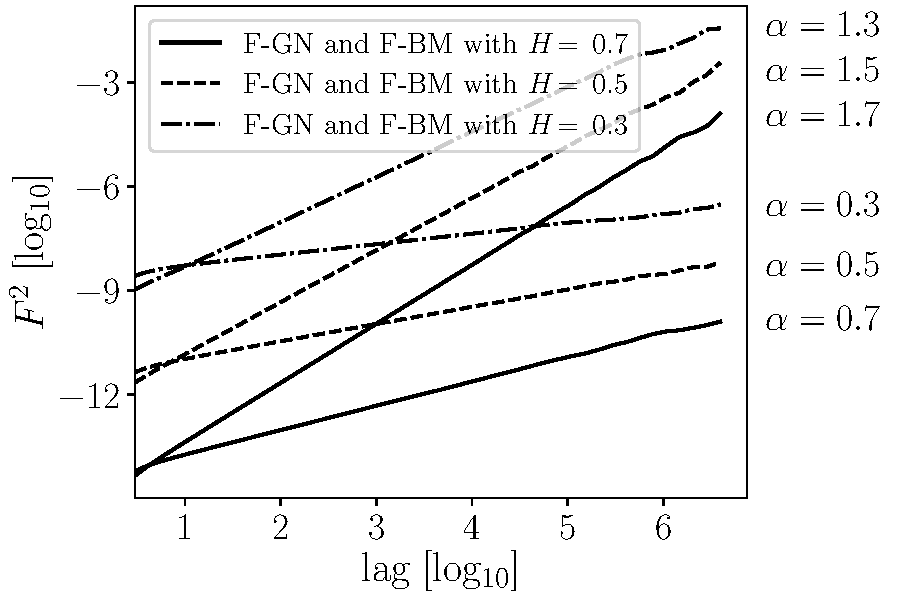
\includegraphics[width = 0.5\linewidth]{fig1.pdf}
  \caption{Multifractal Detrended Fluctuation Analysis of three examplary paths of fractional Ornstein--Uhlenbeck processes, given by Eq. (1),
  with Hurst indices of $H=0.3, 0.5, 0.7$.
  The self-similarity scalings $\alpha$ are obtained my extracting the slopes of the curves (in a log-log scale).
  Numerically integrated with an integration step $\Delta t = 0.0001$ over $500$ time units ($5\times10^6$ data points)}\label{fig:1}
\end{figure}

\begin{figure}[h]
  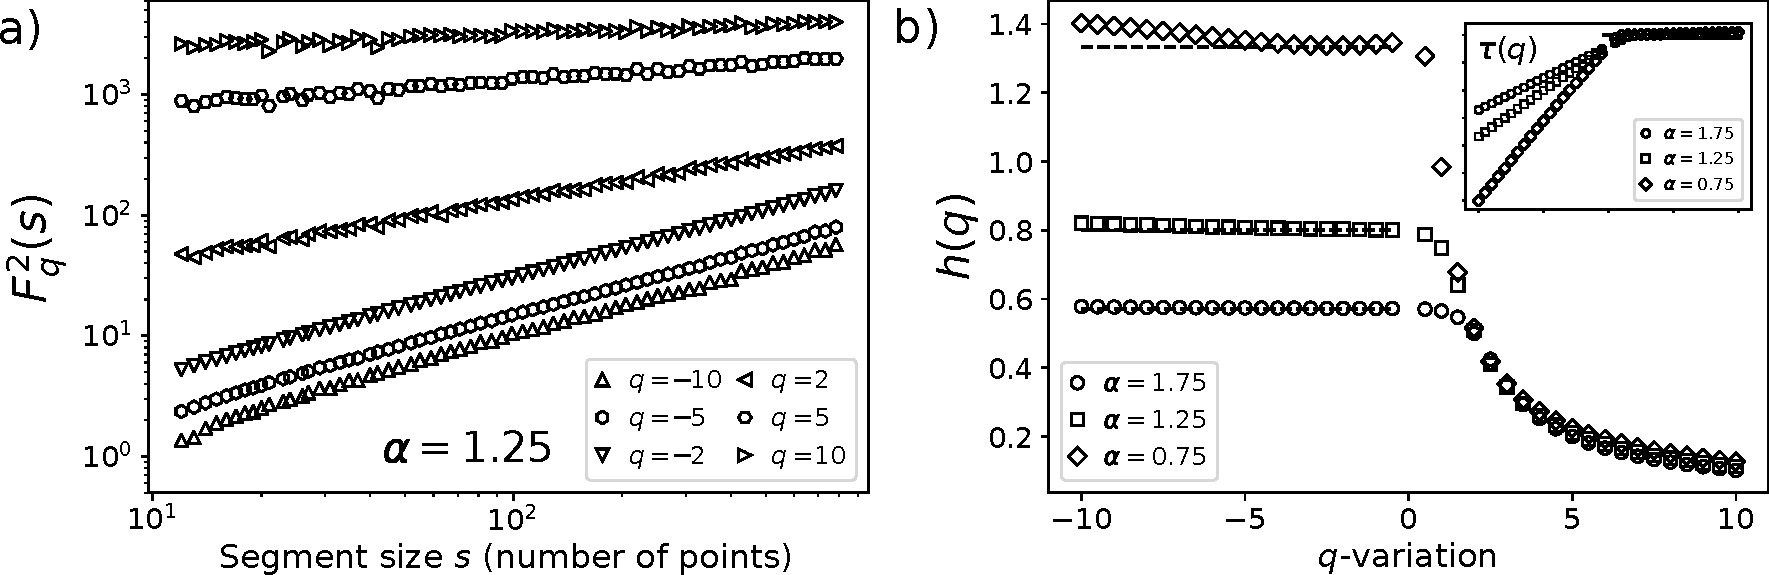
\includegraphics[width = 0.5\linewidth]{fig2.pdf}
  \caption{Multifractal Detrended Fluctuation Analysis of four examplary paths of a fractional Ornstein--Uhlenbeck process with $H=0.7$, fixed $\sigma = 1$, fixed integration timestep $\Delta t = 0.001$, but varying $\lambda = 100, 10, 1,$ and $0.1$ (bottom to top).
  Regardless of the integration timestep, the generalised Hurst exponent $\alpha$ matches the expected value: $\alpha = 0.7$ for $dB_{H=0.7}(t)$, $\alpha = 1.7$ for $B_{H=0.7}(t)$.
  Numerically integrated with an integration step $\Delta t = 0.001$ over $5000$ time units ($5\times10^6$ data points)}\label{fig:2}
\end{figure}

\section{The \texttt{MFDFA} library}
The Multifractal Detrended Fluctuation Analysis library \texttt{MFDFA} presented is a standalone package based integrally on python's \texttt{numpy}, thus it can avail also of \texttt{numpy}'s masked arrays \texttt{ma}, which is particularly convenient when dealing with large datasets with missing data.

The \texttt{MFDFA} library offers a considerable speed-up in comparison with the available Matlab version.
The library is fully developed to work with multithreading, which shows an increase in performance while handling timeseries larger than $10^5$ data points, as seen in Fig.(3).

\begin{figure}[h]
  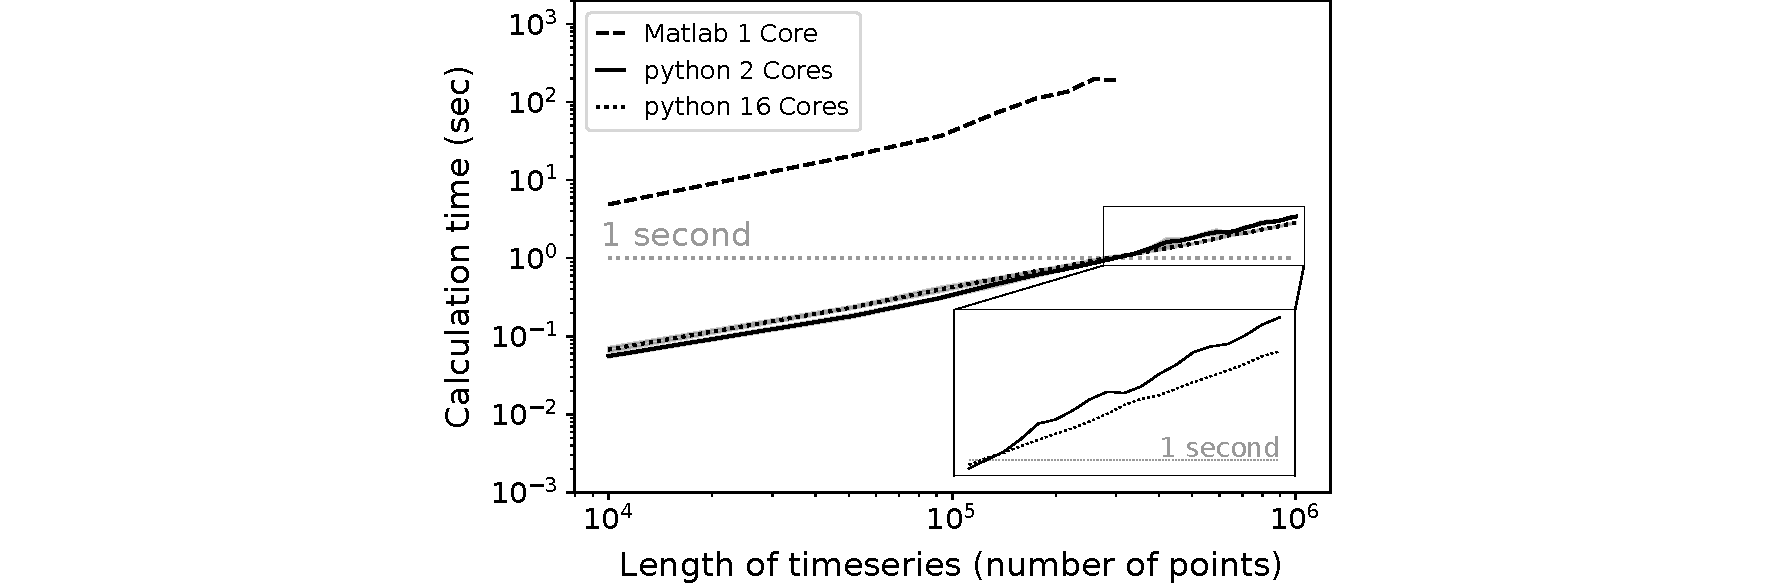
\includegraphics[width = 0.5\linewidth]{fig3.pdf}
  \caption{Performance of \texttt{MFDFA} in comparison with the distributed \texttt{Matlab} version \cite{Ihlen2012}.
  The \texttt{MFDFA} library and \texttt{Matlab} version were tested for a timeseries of a fractional Ornstein--Uhlenbeck with increasing length.
  The \texttt{MFDFA} library is also tested with $2$ and $16$ cores.
  Speed-ups are only noticeable above $10^5$ data points.
  The Matlab code is truncated, since the computation times start exceeding $200$ seconds.}
\end{figure}


\section*{Acknowledgements}
I'd like to thank Fabian Harang, Marc Lagunas, Anton Yurchenko-Tytarenko, Dennis Schroeder, Michele Giordano, Giulia di Nunno and Fred Espen Benth for all the help in understanding stochastic processes, Dirk Witthaut for the support, and Marieke Helmich for the text reviews.
I gratefully acknowledges support by the Helmholtz Association, via the joint initiative \textit{Energy System 2050 - A Contribution of the Research Field Energy}, the grant No. VH-NG-1025, the scholarship funding from \textit{E.ON Stipendienfonds}, and the \textit{STORM - Stochastics for Time-Space Risk Models} project of the Research Council of Norway (RCN) No. 274410, under the supervision of Giulia di Nunno.

\bibstyle{unsrt}
\bibliography{bib}
\end{document}
